We want to implement and apply a soft-margin SVM to the MNINST dataset.\\

First we build a classifier for distinguishing between digits "0" and "1", we tests this with the first 250, 500, and 1000 occurences of the digits from the trainset. Here we apply soft-mmargin SVM with $C= [10^{-6},10^{-5},10^{-4},10^{-3},10^{-2},10^{-1},1,10,100]$, for these we want to provide a graph of $E_{in}$, $||w||$, and $E_{test}$ as a function of $C$, here $E_{test}$ is calculated with the first 1000 occurences of the numbers in the test set. This can be seen in Figure \ref{jegerhomo}.
\begin{figure}
  \centering
  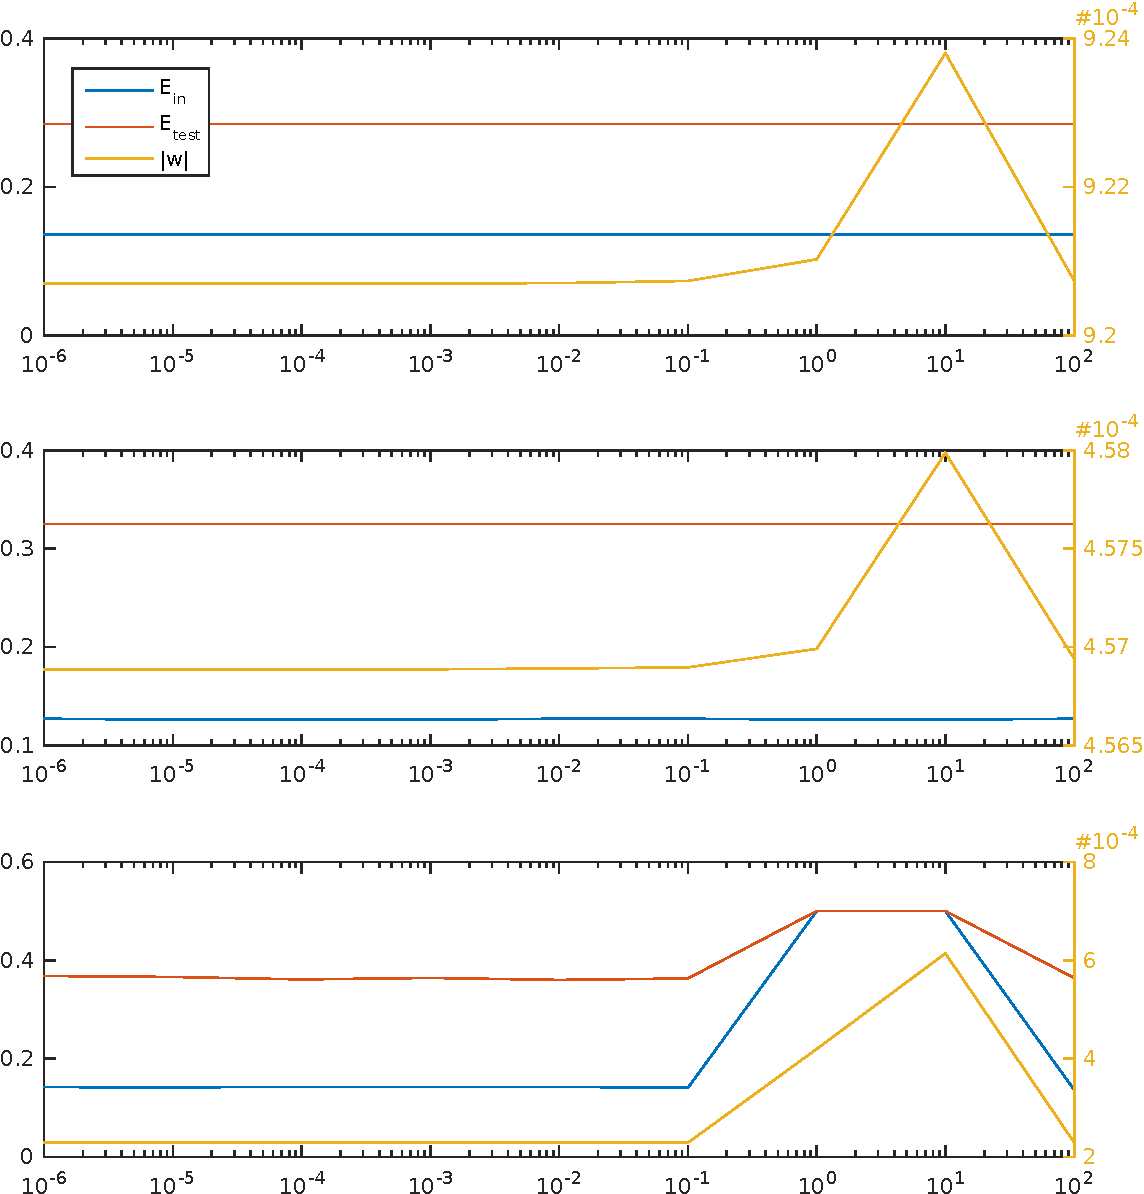
\includegraphics[width=\textwidth]{./01.pdf}
  \caption{$E_{in}$, $||w||$, and $E_{test}$ as a function of $C$, for the first 250, 500, and 1000 occurences of "1" and "0" in the dataset, the top graph is for 250, then 500 and at the bottom 1000.}
  \label{jegerhomo}
\end{figure}
\noindent We do the same for the digits "0" and "8", this can be seen in Figure \ref{sutminfedepik}.
\begin{figure}
  \centering
  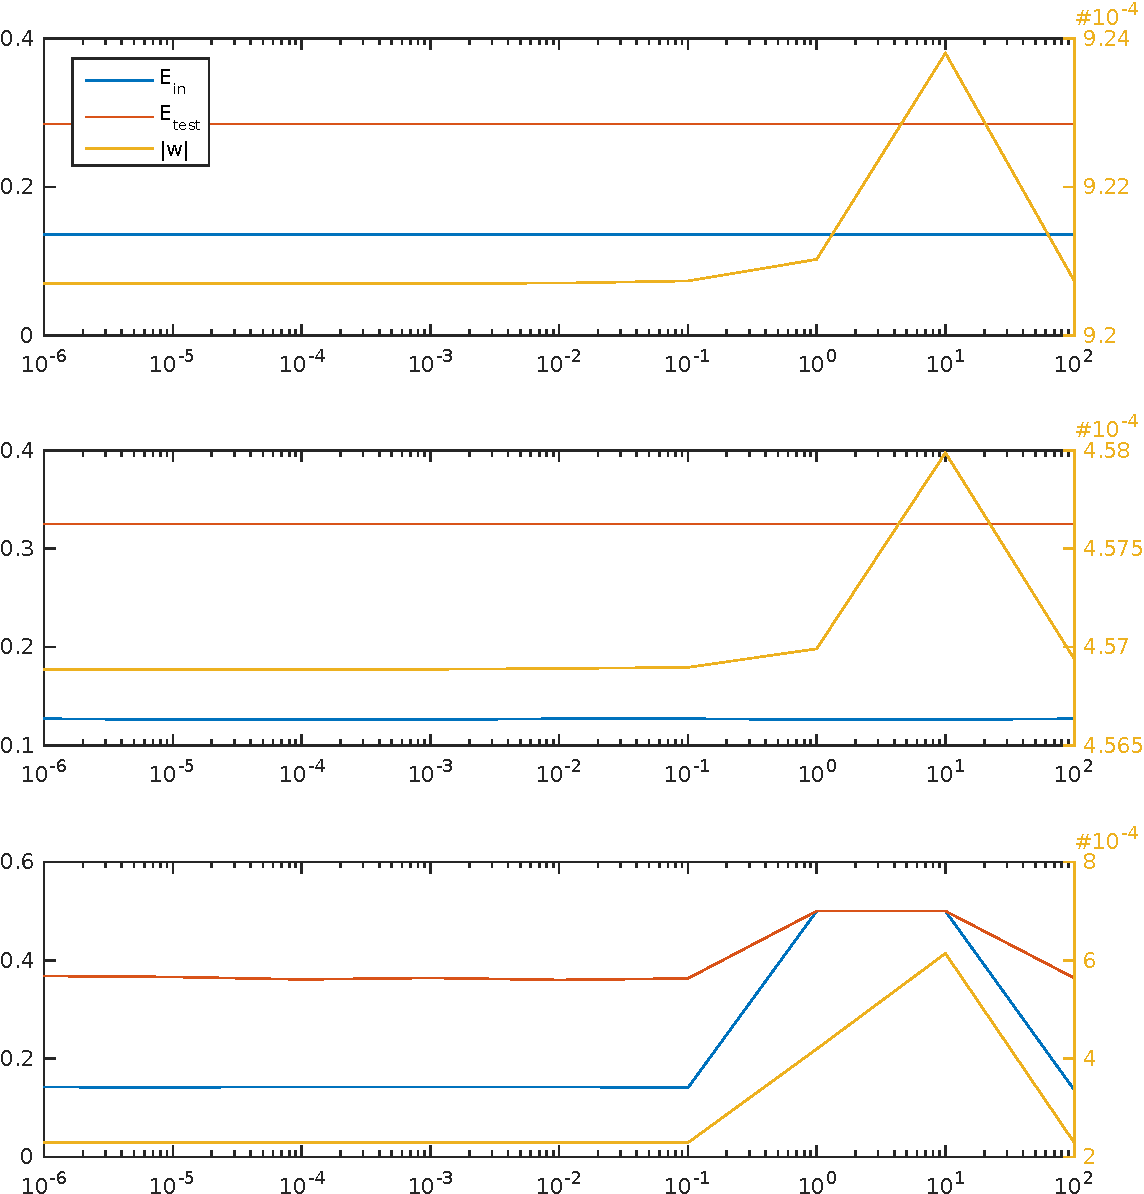
\includegraphics[width=\textwidth]{./08.pdf}
  \caption{$E_{in}$, $||w||$, and $E_{test}$ as a function of $C$, for the first 250, 500, and 1000 occurences of "8" and "0" in the dataset, the top graph is for 250, then 500 and at the bottom 1000.}
  \label{sutminfedepik}
\end{figure}
\noindent We do the same for the digits "5" and "6", this can be seen in Figure \ref{dueretulideligtmenneske}.
\begin{figure}
  \centering
  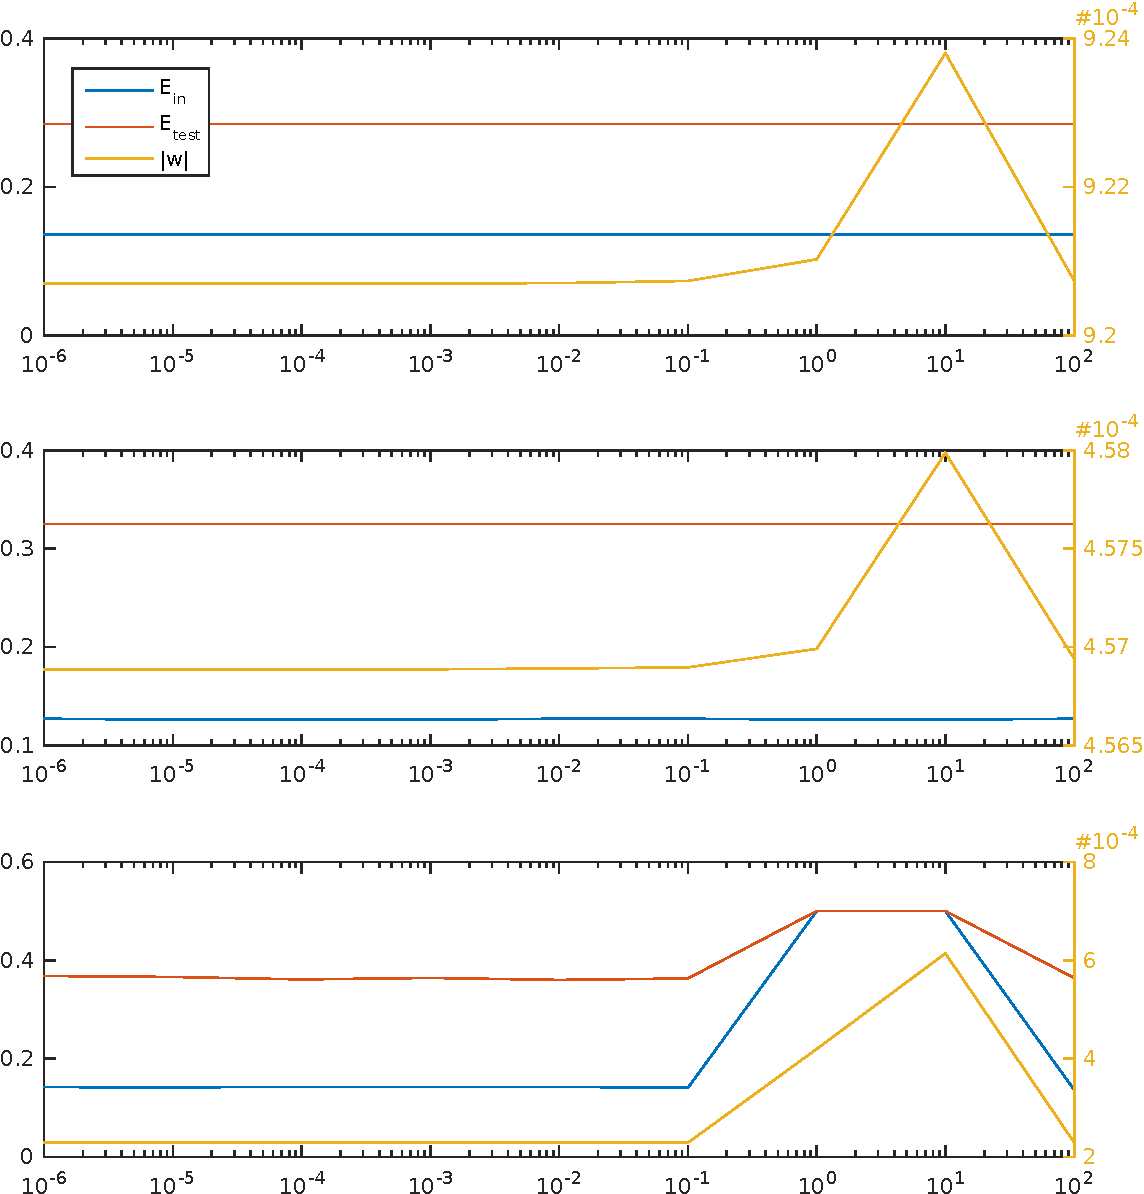
\includegraphics[width=\textwidth]{./56.pdf}
  \caption{$E_{in}$, $||w||$, and $E_{test}$ as a function of $C$, for the first 250, 500, and 1000 occurences of "5" and "6" in the dataset, the top graph is for 250, then 500 and at the bottom 1000.}
  \label{dueretulideligtmenneske}
\end{figure}

